\documentclass[12pt]{article}
\usepackage{graphicx}
\usepackage[margin=1.5in]{geometry}
\usepackage{fullpage}
\usepackage{wrapfig}
\usepackage[colorlinks]{hyperref}
\usepackage{float}

\usepackage{tikz}
\usetikzlibrary{shapes.geometric, arrows}

\tikzstyle{startstop} = [rectangle, rounded corners, minimum width=3cm, minimum height=1cm,text centered, draw=black, fill=red!30]


\tikzstyle{io} = [trapezium, trapezium left angle=70, trapezium right angle=110, minimum width=3cm,,minimum height=1cm,text width=3cm, text centered, draw=black, fill=blue!30]

\tikzstyle{process} = [rectangle, minimum width=3cm,text width=3cm, minimum height=1cm, text centered, draw=black, fill=orange!30]
\tikzstyle{decision} = [diamond, minimum width=3cm,text width=3cm, minimum height=1cm, text centered, draw=black, fill=green!30]

\tikzstyle{arrow} = [thick,->,>=stealth]





\begin{document}




\begin{center}
\textbf{\LARGE  Assignment No.- 6} 
\end{center}

\begin{center}
\textbf{\LARGE ELP - 718 Telecom Software Lab }
\end{center}
\begin{center}

\end{center}
\begin{center}
\textbf{\large  Bhawna Kamra}
\end{center}
\begin{center}
\textbf{\large 2017JTM2187 }
\end{center}
\begin{center}
\textbf{\large Semester-1 }
\end{center}


\begin{center}

\end{center}
\begin{center}

\end{center}






\centering
A report presented for the assignment
Developing logical skills to solve the given problem with the help of basic C.




\begin{center}

\end{center}

\begin{center}

\end{center}



\begin{figure}[H]
\center
\includegraphics[scale=0.5]{images.png}
    
    
\end{figure} 

\begin{center}

\end{center}
\begin{center}

\end{center}

\begin{center}
Bharti School  \\
Telecommunication Technology and Management  \\
IIT DELHI  \\
India  \\

August 2, 2016

\end{center}

  
\newpage
\tableofcontents
\pagebreak
\begin{flushleft}


\section{ Problem statement 1}

\end{flushleft}
\begin{flushleft}
\textbf{Parity Check:\\}
The simplest way of error detection is to append a single bit , called a parity check, to a string of data bits. This parity check bit has the value 1 if number of 1’s in the bit string is even and has the value 0 otherwise, i.e., Odd Parity Check.

\textbf{Bit Oriented Framing:\\}
Data Link Layer needs to pack bits into frames, so that each frame is distinguishable from another. Frames can be fixed or variable size. In variable size framing, we define end of frame using bit oriented approach. It uses a special string of bits, called a flag for both idle fill and to indicate the beginning and the ending of frames.
The string 0101 is used as the bit string or flag to indicate the end of the frame. The bit stuffing rule is to insert a 0 after each appearance of 010 in the original data. In addition, if the frame ends in 01, a 0 would be stuffed after the 1st 0 in the actual terminating string 0101.








\end{flushleft}

\begin{flushleft}


\subsection{Assumptions}
\begin{flushleft}
The information wwe are going to use ,we have already stored that in the file.
\end{flushleft}


\end{flushleft}



\begin{flushleft}


\subsection{Structure Chart}
\begin{center}

\end{center}
\end{flushleft}

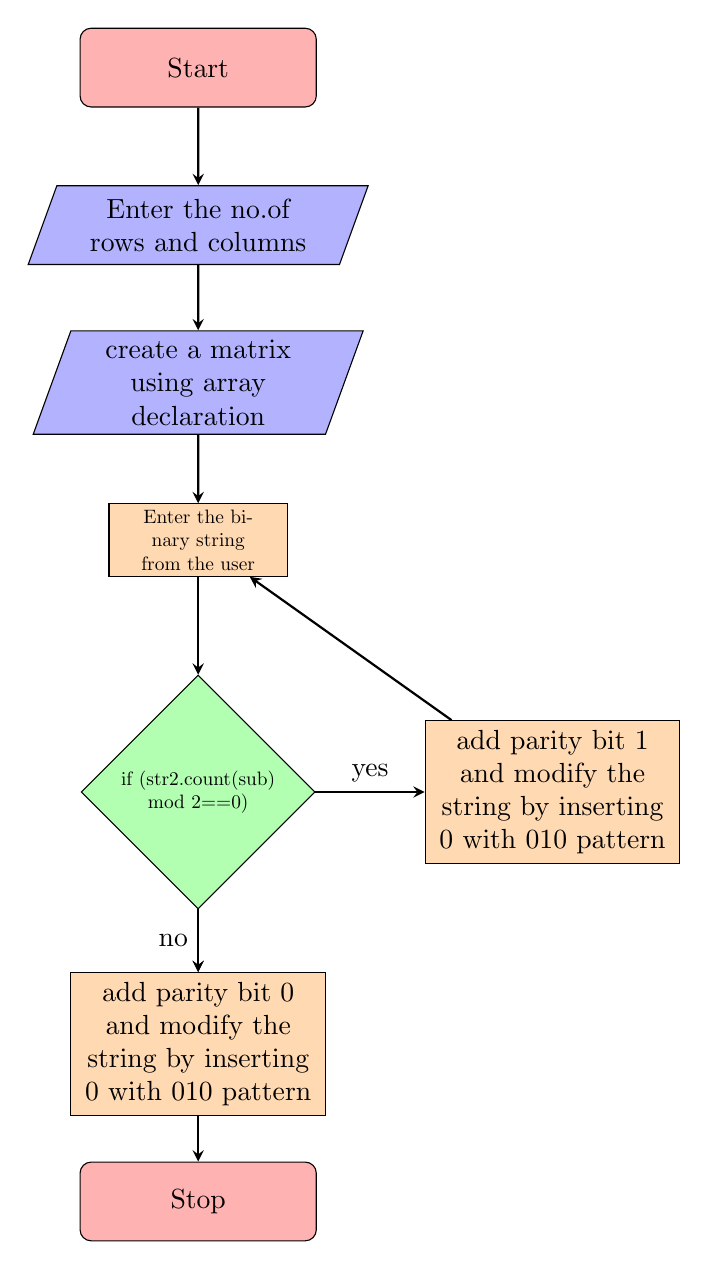
\begin{tikzpicture}[node distance=2cm]

\node (start) [startstop] {Start};

\node (in1) [io, below of=start] {Enter the no.of rows and columns};

\node (in2) [io, below of=in1] {create a matrix using array declaration};




\node (pro1) [process, below of=in2,scale=0.7] {Enter the binary string from the user};
\node (dec1) [decision, below of=pro1,yshift=-1.2 cm,scale=0.7] {if (str2.count(sub) mod 2==0)};
\node (pro2a) [process, right of=dec1,xshift=2.5 cm] {add parity bit 1 and modify the string by inserting 0 with 010 pattern};


\node (pro2) [process, below of=dec1,yshift=-1.2 cm] {add parity bit 0 and modify the string by inserting 0 with 010 pattern};

\node (stop) [startstop , below of=pro2] {Stop};


\draw [arrow] (start) -- (in1);
\draw [arrow] (in1) -- (in2);
\draw [arrow] (in2) -- (pro1);
\draw [arrow] (pro1) -- (dec1);
\draw [arrow] (dec1) -- (pro2);

\draw [arrow] (pro2a) --(pro1);

\draw [arrow] (pro2) -- (stop);


\draw [arrow] (dec1) -- node[anchor=south] {yes} (pro2a);
\draw [arrow] (dec1) -- node[anchor=east] {no} (pro2);











\end{tikzpicture}
\begin{flushleft}

\section{  Implementation}

\subsection{Input Format}
\begin{flushleft}
Enter binary bit data which has to be transmitted.



\end{flushleft}


\subsection{ Output Format}
\begin{flushleft}

Print binary bit data with parity bit.
Print the modified string received at the other end.

\end{flushleft}





\section{ Test Description}

Sample Input:
01010

 
Sample Output:
010101
0100100100101


\section { Screenshots}





\end{flushleft}














\end{document}
